% 第 3 章 §3.4 前半（印刷页 137–144）

\section{一维与二维的配边假设}

所谓「配边假设」（cobordism hypothesis），是指关于取值为任意对称幺半 $D$-范畴的全扩展 $D$ 维 TQFT 的分类。它由 Baez--Dolan [5] 提出（并不完全精确）：粗略地说，这样一个理论应当由该 $D$-范畴中赋值给一个点的对象完全决定；该对象必须满足某些条件，并带有额外的结构。Lurie [19] 把这两方面都精确化，并证明了这一猜想。他的表述背后的关键洞见（使之区别于 [23] 等其他变体）在于把条件与结构分离开来。

这通过过渡到标架配边 $D$-范畴（framed bordism $D$-category）$\mathsf{Bord}^{\mathrm{fr}}_D$ 来实现，其定义见下。此时，赋值给点的对象 $Z(*)$ 受制于完全可对偶性（full dualizability）条件，后者在 $D=1$ 的情形推广了向量空间的有限维性。这里没有额外的结构；后者只在试图借助带有其他结构（定向、spin，或切丛上任何由拓扑定义的结构）的流形来分解一个标架理论时才出现。

同样粗略地说，要把如上所述的标架理论从标架流形推广到这样一个流形范畴——其切丛的拓扑结构群从正交群约化为某个群 $G\to\mathrm{O}(D)$——就需要把对象 $Z(*)$ 做成 $G$-等变的。更精确地说，需要把 $Z(*)$ 展示为目标 $D$-范畴中所有可对偶对象构成的空间里的一个 $G$-不动对象，这里用的是该空间上典范的 $\mathrm{O}(D)$ 作用。

让我们从一个定义的开头讲起，它掩盖了不完整之处与许多精细之处；我们将从下面的注记开始，逐步把它们解开。

\begin{definition}\label{def:3.4.1}
流形 $M$ 上 $n$ 维向量丛 $V$ 的一个标架（framing）是 $V$ 与平凡向量丛 $M\times\R^n$ 的一个同构。光滑 $k$-流形 $M$（其中 $k\le D$）上的一个 $D$-标架，是丛 $\R^{D-k}\oplus TM$ 的一个标架。
\end{definition}

$D$-范畴 $\mathsf{Bord}^{\mathrm{fr}}_D$ 以 $D$-标架的点为对象，其 $k$-态射是紧的带角 $D$-标架流形。对 $k=D$，我们取 $D$-流形，模去固定边界的微分同胚与标架的同伦。

\begin{remark}[标架]\label{rem:3.4.2}
\begin{enumerate}[label=(\roman*),leftmargin=3em]
\item 重要的是，标架中多出来的那些 $\R$ 不必与 $\R^D$ 的前几个直和项对齐；否则我们所定义的只不过是 $TM$ 的普通标架。$D$-标架与稳定标架（即允许 $D$ 任意大的概念）相近，但略具限制性。当 $\dim M<D-1$ 时，$D$-标架成为稳定的，其原因在于 $\mathrm{SO}$ 的同伦群的稳定化。
\item 设 $B$ 是 $M$ 的边界的一个 $(k-1)$ 维分支，则 $TM|_B$ 有一个 $\R^1$ 直和项，它可以用 $B$ 在 $M$ 中的内向或外向法向标架化。这一选择给出同构 $\R^{D-k}\oplus TM|_B\cong\R^{D-k+1}\oplus TB$。$\R^1$ 上的方向依我们把 $B$ 读作态射 $M$ 的源还是靶而定，而 $M$ 的 $D$-标架随即限制为 $B$ 的一个 $D$-标架。一旦我们把 $M$ 读作态射之间的态射（以及态射之间的态射之间的态射，……），就可以一致地把这一约定沿所有余维数贯彻下去，从而构造出 $D$-标架流形的 $D$-范畴。
\item 带角的 $D$-标架流形可以以多种方式读作态射：其各种余维数的边界必须标注为态射的源或靶。例如，图 3.1 展示了一个方形的四种读法，即把它读作各种 1-态射的恒等 2-态射。1-态射从右向左，2-态射向下。标架标在曲面上，角点的符号由我们的标架约定强制决定：角点处的切空间 $TM$ 以（2-态射，1-态射）给出的基为准，再与曲面标架作比较。竖线始终是角对象的自身等同。还有多得多的可能性，因为 2-标架不必如这里所画的那样沿水平方向为常值；事实上，标架的一个单位扭转将扮演特殊的角色（Serre 自同构）。
\item 对 $D>0$，$\mathsf{Bord}^{\mathrm{fr}}_D$ 中恰有两个 $D$-标架的点 $+$、$-$（同构意义下），它们由标架 $\R^D\cong\R^D\oplus T(\text{point})$ 的行列式符号区分。这一同构由同一定向类中从一个标架到另一个标架的任意同伦实现，该同伦看作一个 $D$-标架的区间（$\mathsf{Bord}^{\mathrm{fr}}_D$ 中的一个 1-态射）。相反方向的同伦给出逆同构（相差可逆的 2-态射，等等）。每个标架的点的自同构群是 $\Omega\mathrm{SO}(D)$。
\end{enumerate}
\end{remark}

\begin{figure}[htbp]
\centering
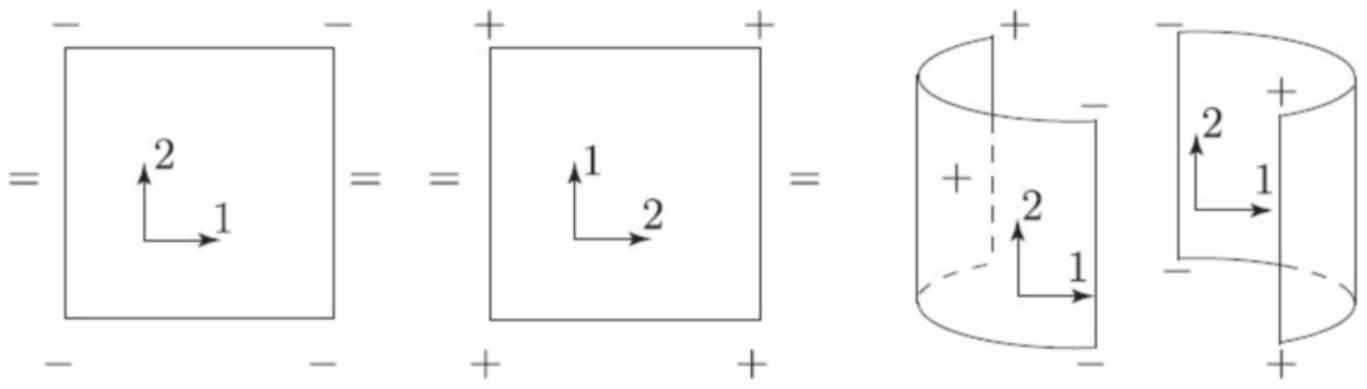
\includegraphics[width=360.9pt]{figs/f3-01.png}
\caption{方形的各种 2-态射读法}
\label{fig:3.1}
\end{figure}

\begin{remark}[微分同胚]\label{rem:3.4.3}
在最高维模去微分同胚，在有经验的读者看来是不对的：这是因为微分同胚群带有拓扑，而朴素的定义把这一拓扑丢掉了。例如，这样的定义永远无法捕捉 Gromov--Witten 理论的结构，因为后者依赖于 $\overline{\mathcal{M}}^n_g$ 的拓扑。相反，每个最高维流形都应换成一个态射空间，其同伦型为相应的 $B\mathrm{Diff}$。\footnote{再加上相对于边界的标架空间。} 实现这一点的首选方式涉及 $(\infty,D)$-范畴的概念：它对所有 $k$ 都有有意思的 $k$-态射，但要求 $D$ 以上的一切都是同构。$B\mathrm{Diff}$ 的同伦型于是被 $D$-态射的更高自同构群捕捉。
\end{remark}

\subsection{对偶与一维标架 TQFT}

对 $\R$-丛而言，标架与定向在相差一个可缩的选择空间的意义下一致。回忆一下：有向理论由赋值给两个有向点的向量空间 $Z(+)$、$Z(-)$，以及映射
\begin{equation}
\begin{gathered}
Z(\mathord{\supset})\colon \C\longrightarrow Z(-)\otimes Z(+),\\
Z(\mathord{\subset})\colon Z(+)\otimes Z(-)\longrightarrow \C
\end{gathered}
\tag{3.5}\label{eq:3.5}
\end{equation}
组成。它们受制于如下条件：复合
\begin{equation}
\begin{gathered}
Z(+)\xrightarrow{\ \Id\otimes Z(\mathord{\subset})\ }Z(+)\otimes Z(-)\otimes Z(+)\xrightarrow{\ Z(\mathord{\supset})\otimes\Id\ }Z(+),\\
Z(-)\xrightarrow{\ Z(\mathord{\subset})\otimes\Id\ }Z(-)\otimes Z(+)\otimes Z(-)\xrightarrow{\ \Id\otimes Z(\mathord{\supset})\ }Z(-)
\end{gathered}
\tag{3.6}\label{eq:3.6}
\end{equation}
分别是相应的恒等映射。这些条件在几何上可以通过把两个半圆在相应的端点粘合而看出：我们得到一个「S」形或「Z」形，它们都微分同胚于恒等区间（见图 3.2）。

\begin{annote}
底本 §3.1.3（印刷页 111）把右弧写作 $Z(\mathord{\supset})\colon\C\to Z(+)\otimes Z(-)$，与本节式 (3.5) 的因子次序相反；两处均照底本排印。在对称幺半范畴中二者经换位同构等同，不影响后文。
\end{annote}

\begin{figure}[htbp]
\centering
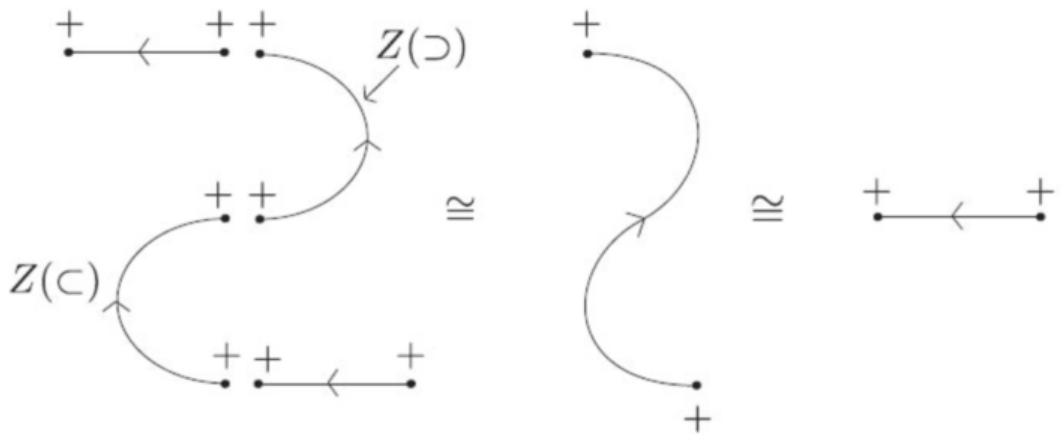
\includegraphics[width=280.9pt]{figs/f3-02.png}
\caption{Zorro 引理}
\label{fig:3.2}
\end{figure}

\begin{definition}[幺半范畴中的内部对偶]\label{def:3.4.4}
在幺半范畴中，给定如 (3.5)--(3.6) 的一对对象与态射（以单位对象代替 $\C$），我们称 $Z(+)$ 是 $Z(-)$ 的右对偶，$Z(-)$ 是 $Z(+)$ 的左对偶。此外，$Z(\mathord{\subset})$ 与 $Z(\mathord{\supset})$ 分别称为该伴随的单位与迹。
\end{definition}

\begin{annote}
按式 (3.5)，由 $\C$ 出发的 $Z(\mathord{\supset})\colon\C\to Z(-)\otimes Z(+)$ 是余求值，即伴随的单位；而 $Z(\mathord{\subset})\colon Z(+)\otimes Z(-)\to\C$ 是求值，即迹。底本此句把两者的配对次序写反，今照底本排印并记于此。
\end{annote}

\begin{remark}[对偶性]\label{rem:3.4.5}
\begin{enumerate}[label=(\roman*),leftmargin=3em]
\item 给定对象的左对偶（若存在）连同单位/迹，被典范地确定到同构为止。
\item 强化这一陈述：有对偶的对象之间的态射有一个伴随态射，以相反方向联系它们的对偶。
\item 可逆对象总有对偶：其逆即可取作对偶。
\item（Hom 定义）对偶性的等价定义是：指定一个关于 $x,y$ 双函子性的同构 $\Hom(x\otimes Z(-),y)\cong\Hom(x,y\otimes Z(+))$。换言之，函子 $\cdot\otimes Z(-)$ 与 $\cdot\otimes Z(+)$ 构成伴随对；见下文 §3.4.4。
\item 在对称幺半范畴中，左对偶与右对偶是等价的条件；此时可把 $x$ 的对偶记作 $x^\vee$。但后面在考虑更高范畴中的 $\Hom(\ ,\ )$ 范畴时，我们仍会遇到左/右的区分。
\item 向量空间恰在有限维时才有对偶。交换环上有限生成投射模有对偶，但在一般环上，它们并不是唯一有对偶的模。
\end{enumerate}
\end{remark}

\subsection{一维的配边假设}

若对称幺半范畴中的一个对象确有对偶，则称之为可对偶的（dualizable）。我们刚刚看到，到某个对称幺半范畴 $\mathcal{C}$ 的函子 $Z\colon\mathsf{Bord}^{\mathrm{fr}}_1\to\mathcal{C}$，在同构意义下由 $Z(+)$ 分类，而 $Z(+)$ 是 $\mathcal{C}$ 中的可对偶对象。

一个值得做的练习是证明：函子的任何自然变换 $Z\to Z'$ 都是同构，特别地来自一个同构 $f\colon Z(+)\to Z'(+)$。（证明：相伴态射 $g\colon Z(-)\to Z'(-)$ 必是伴随态射 $f^\vee$ 的逆；因此 ${}^\vee g$ 将是 $f$ 的逆。）

\subsection{可对偶对象上的 O(1) 作用}

正交群 $\mathrm{O}(D)$ 通过改变标架作用于 $\mathsf{Bord}^{\mathrm{fr}}_D$。这是一个同伦意义下的作用：它穿过群的同伦型，对 Lie 结构不敏感（见注 3.4.13）。因此它作用于标架 TQFT，从而作用于可能的 $Z(+)$ 的集合，即给定对称张量范畴中允许对偶的那些对象。在对象上的作用是显然的，它穿过 $\{\pm1\}$：非平凡元把每个这样的对象送到它的对偶。

那么，理论何时穿过无定向流形？此时 $+=-$，故可取 $Z(+)=Z(-)$。于是 $Z(\mathord{\subset})$ 是一个非退化配对 $Z(+)\otimes Z(+)\to\mathbf{1}$。$\mathord{\subset}$ 上没有定向迫使它对称，所以在向量空间上，理论由一个带非退化对称双线性型的向量空间决定。

下面给出内蕴的描述。群 $\Z/2\Z$ 作用于有限维复向量空间与同构构成的群胚（记作 $G_{>0}\mathsf{Vect}$），把向量空间送到其对偶，把线性同构送到其逆对偶。这就是 $\mathrm{O}(1)$ 在 $\mathsf{Vect}$ 的可对偶对象上的作用。（我们看到需要把范畴截断为其极大子群胚：在整个子范畴上，这个作用定义不良。）在解释它之前，先陈述下面的命题。

\begin{proposition}\label{prop:3.4.6}
这个 $\mathrm{O}(1)$-作用的不动点范畴是带非退化对称双线性型的向量空间构成的群胚。特别地，无定向 TQFT 由 $\mathsf{Vect}$ 中可对偶对象之间的 $\mathrm{O}(1)$-不动点分类。
\end{proposition}

首先，我们说一个（离散）群 $G$ 作用在范畴 $\mathcal{C}$ 上，是指：对每个元素 $g\in G$，给定一个自函子 $F_g\colon\mathcal{C}\to\mathcal{C}$；并且对所有 $g,h$，给定函子的同构 $\alpha_{g,h}\colon F_g\circ F_h\xrightarrow{\sim}F_{gh}$，使得三元组 $g,h,k$ 中的诸 $\alpha$ 满足显然的融贯关系，从而使我们能构造出唯一的同构 $F_g\circ F_h\circ F_k\cong F_{ghk}$。此外，不妨设 $F_1=\Id$。

不动点范畴 $\mathcal{C}^G$ 按定义是这样一个范畴：其对象是元组 $(x,\varphi_{x,g}|_{g\in G})$，其中 $\varphi_{x,g}\in\operatorname{Isom}(x,F_g(x))$ 关于复合满足一个（显然的）融贯约束：$\varphi_{x,gh}=F_g(\varphi_{x,h})\circ\varphi_{x,g}$（忽略诸 $\alpha$）。也就是说，我们能找到的把 $x$ 与 $F_{gh}(x)$ 等同起来的两种方式一致。$\mathcal{C}^G$ 中的态射来自 $\mathcal{C}$，但要求与诸 $\varphi$ 相容。

现在，证明下面的事实是一个练习：对 $\mathrm{O}(1)$ 的非平凡元 $g$，只需指定一个 $\varphi\colon V\to V^\vee$。条件 $g^2=1$ 蕴涵 $(\varphi^\vee)^{-1}\circ\varphi=\Id_V$，即 $\varphi$ 的对称性。

\subsection{二维的配边假设}

我们回顾更高范畴中态射的伴随概念，它是对象对偶的类比物。幸运的是，此后的所有更高定义都将是一样的。关键的例涉及范畴之间的函子：若给定双函子性的同构 $\Hom_{\mathcal{C}}(x,Gy)=\Hom_{\mathcal{D}}(Fx,y)$，我们称 $F\colon\mathcal{C}\rightleftarrows\mathcal{D}:G$ 构成伴随对，$F$ 为左伴随、$G$ 为右伴随。显然，$F$ 的右伴随（若存在）在同构意义下唯一；记 $G=F^\vee$。类似地，左伴随 $F$ 由 $G$ 唯一确定（到同构为止），记 $F={}^\vee G$。

取 $y=Fx$ 给出单位态射 $\varepsilon\colon\Id_{\mathcal{C}}\to G\circ F$；取 $x=Gy$ 给出迹 $\theta\colon F\circ G\to\Id_{\mathcal{D}}$。借助 $\varepsilon$ 与 $\theta$，我们可以在不涉及 $\mathcal{C}$ 与 $\mathcal{D}$ 中对象的情况下陈述伴随条件。

\begin{definition}\label{def:3.4.7}
2-范畴中的态射 $F\colon c\to d$ 是 $G\colon d\to c$ 的左伴随，若存在单位 2-态射 $\varepsilon\colon\Id_c\to G\circ F$ 与迹（或称求值）$\theta\colon F\circ G\to\Id_d$，使得下列复合分别是相应的恒等 2-态射：
\begin{gather*}
F=F\circ\Id_c\xrightarrow{\ \Id_F\otimes\varepsilon\ }F\circ G\circ F\xrightarrow{\ \theta\otimes\Id_F\ }\Id_d\circ F=F,\\
\Id_c\circ G=G\xrightarrow{\ \varepsilon\otimes\Id_G\ }G\circ F\circ G\xrightarrow{\ \Id_G\otimes\theta\ }G\circ\Id_d=G.
\end{gather*}
此时称 $G$ 是 $F$ 的右伴随。
\end{definition}

一个态射称为可对偶的，若它有右伴随与左伴随，而后者又有右伴随与左伴随，如此以至无穷。

\begin{remark}\label{rem:3.4.8}
\begin{enumerate}[label=(\roman*),leftmargin=3em]
\item 那个无意义却简洁的公式「$\theta\circ\varepsilon=1$」恰可按上述两种方式赋予意义。
\item 我们可以借助诱导的变换 $F_*\colon\Hom_{\mathcal{C}}(\bullet,c)\rightleftarrows\Hom_{\mathcal{C}}(\bullet,d):G_*$ 回到伴随的 Hom 定义，即要求在 $\mathcal{C}$ 上的范畴值函子之间，$F_*$ 与 $G_*$ 互为伴随（关于 $\bullet$ 函子性地）。
\item 可对偶性的定义似乎包含无穷多个条件。然而在 TQFT 的应用中，条件将是有限多个。这是因为左伴随与右伴随必须相差一个可逆函子（二维情形即 Serre 自同构），而一旦找到该函子并验证其可逆性，检验便可停止：所有进一步伴随的存在性由此得到保证。
\item 注意，若 $\varepsilon$、$\theta$ 是同构，则 $F$ 与 $G$ 也是同构，且互为逆。
\end{enumerate}
\end{remark}

\begin{definition}\label{def:3.4.9}
对任意 2-范畴 $\mathcal{C}$，记 $G_{>1}\mathcal{C}$（「1-态射之上的群胚」）为保留所有对象与 1-态射、但只保留可逆 2-态射的 2-范畴。\footnote{若从 $(\infty,2)$-范畴出发，这样得到的是一个 $(\infty,1)$-范畴。} 对任意 $D$-范畴（$D>k$）有类似的定义 $G_{>k}\mathcal{C}$。
\end{definition}

\begin{definition}\label{def:3.4.10}
对称幺半 $(\infty,2)$-范畴中的对象 $x$ 称为完全可对偶的（fully dualizable），若它在 $G_{>1}\mathcal{C}$ 中可对偶，且其对偶的单位与迹在各自相应的函子 1-范畴中可对偶。
\end{definition}

\begin{remark}\label{rem:3.4.11}
我们不要求进一步的对偶，因为 2 以上只有同构。坚持要求更多的对偶会迫使一切（包括 $x$）可逆。（展开 3.4.8.iv。）
\end{remark}

\begin{theorem}[标架 TQFT 的分类]\label{thm:3.4.12}
取值于 2-范畴 $\mathcal{C}$（或 $(\infty,2)$-范畴）的二维标架扩展 TQFT $Z$ 由 $x=Z(+)$ 决定，而 $x$ 可以是任意完全可对偶对象。

两个理论 $Z_x$ 与 $Z_y$ 之间的自然变换构成一个（2-）群胚（或 $\infty$-群胚），它等价于范畴 $G_{>0}\mathcal{C}$（由 $\mathcal{C}$ 只保留可逆 1-态射与 2-态射而得）中的 $\Hom(x,y)$。
\end{theorem}

\subsection{Serre 扭转}

设 $x$ 是完全可对偶对象，对偶为 $x^\vee$；称 $u$、$ev$ 分别为该对偶的单位与迹。又设 $S\colon Z(+)\to Z(+)$ 为 Serre 自同构，它由沿区间的标架作顺时针扭转而诱导（图示见 §3.4.8）。我们将看到，在 $\mathsf{Bord}^{\mathrm{fr}}_2$ 中，$(S\boxtimes\Id_-)\circ u$ 是 $ev$ 的右伴随，而 $(S^{-1}\boxtimes\Id_-)\circ u$ 是 $ev$ 的左伴随。其余的伴随由此代数地确定，因为 $S^{-1}=S^\vee$（左伴随与右伴随）。特别地，这证明了配边假设的一半，即 $Z(+)$ 必须是完全可对偶的。另一半（也是更难的一半）是如下陈述：$\mathsf{Bord}^{\mathrm{fr}}$ 是由一个完全可对偶对象生成的自由 2-范畴；换言之，没有额外的关系需要加在 $Z(+)$ 上。

\begin{remark}\label{rem:3.4.13}
对 $S$ 的等价描述始于如下观察：$\Aut(+)\simeq\Omega\mathrm{SO}(2)\simeq\Z$，而 $S$ 是负生成元。完全可对偶对象上的 $\Z$-作用捕捉了 $\mathrm{SO}(2)$ 在全体完全可对偶对象构成的空间上的拓扑作用：因为 $\mathrm{SO}(2)$ 连通，对任意完全可对偶的 $x$ 有 $gx\cong x$；同构的选取来自从 $1$ 到 $g$ 的任意道路的选取，且对道路的形变不敏感。然而，若想融贯地把这些同构「拉直」，以平凡化 $x$ 的轨道上的作用，则恰好受到自同构 $S$ 的阻碍，而 $S$ 来自 $\mathrm{SO}(2)$ 中的非平凡环路。
\end{remark}

\subsection{有向理论与 r-Spin 理论}

有了 Serre 自同构，我们现在陈述有向 TQFT 与 Spin TQFT 的分类。更精确地说，我们寻求标架理论穿过有向配边范畴的条件。事实上，对每个 $r$，我们都可以问及带 $r$-Spin 结构的曲面与圆周的 TQFT，$r$-Spin 结构即切丛的一个选定的 $r$ 次根（假定切丛有定向）。$r=1$ 时我们得到有向曲面，$r=2$ 时得到传统的 Spin 结构。

\begin{theorem}\label{thm:3.4.14}
标架理论 $Z\colon\mathsf{Bord}^{\mathrm{fr}}_2\to\mathcal{C}$ 穿过 $r$-Spin 范畴 $\mathsf{Bord}^{r\text{-}\mathrm{Spin}}_2$ 的分解，对应于 $S^r$ 与 $Z(+)$ 的恒等自同构之间的同构。
\end{theorem}

\begin{example}[半单 TQFT]\label{ex:3.4.15}
对 $\C$-线性 TQFT（取值于线性范畴的 2-范畴），Serre 函子的一个给定平凡化可以乘上任意的 $\lambda\in\C^\times$。此时，计算表明闭亏格 $g$ 曲面的不变量 $Z(\Sigma_g)$ 会乘上 $\lambda^{2-2g}$。更精确地说，$Z(S^1)$ 上的 Frobenius 迹 $\theta$ 乘上 $\lambda^2$，而由带一个出边界圆周的环面（有时称为欧拉类）在 $Z(S^1)$ 中定义的向量乘上 $\lambda^{-2}$。

现在回忆，由半单 Frobenius 代数定义的理论给出闭曲面不变量 $Z(\Sigma_g)=\sum\theta_i^{1-g}$。这样的理论可以解释为一维扩展 TQFT 的和，其中每一个由代数 $\C$ 连同 Serre 函子 $\theta_i^{1/2}$ 生成。换言之，闭曲面不变量完全可以追溯到 Serre 自同构的选取，而这一选取可以对每个直和项独立地缩放。然而，要把理论一路向下定义到零维，就要求我们选取 Frobenius 结构常数 $\theta_i$ 的平方根。
\end{example}

\subsection{图示中的伴随：有向把柄}

现在我们把 2-对偶的数据与关系按几何方式逐一写出，用标准的把柄与把柄消去来表述。对 $D=1$，我们在把「Z」形化为区间时已经这样做过，只是它可能太显然而不易察觉。若假设 $S=\Id_+$（此时 TQFT 穿过有向曲面），图形会更少也更简单。此时 $u$ 与 $ev$ 互为左伴随与右伴随，而伴随的单位 $\varepsilon$ 与迹 $\theta$ 就是曲面拓扑中的标准把柄，如图 3.3 所示。

1-态射从右向左读，曲面 2-态射向下读。箭头指示 1-态射区间的定向；曲面的定向由如下规则推出：在边界处，标架中 2-态射的方向排在前面。

% 本节续见 ch03f.tex（§3.4.7 后半，图 3.3 起）
